%In diesem Unterkapitel sollten folgende Punkte behandelt werden:
%\begin{itemize}
%	\item	Was ist das Problem
%	\item 	Problemgeschichte?
%\end{itemize}
\section{Motivation}

\nomenclature[Fachbegriff]{GUI}{Graphical-User-Interface, Grafische Benutzeroberfläche}

In der Welt der Webapplikationen gibt es die Hürde, dass meist keine direkte Kommunikation zwischen Nutzern und den Verantwortlichen besteht. Die Verantwortlichen werden in dieser Arbeit mit \textbf{Stakeholder} bezeichnet und umfassen Betreiber und Entwickler.

Die Stakeholder müssen aber das Nutzer- und das Anwendungsverhalten verstehen und nachvollziehen können. Nur so kann eine effiziente Instandhaltung und erfolgreiche Weiterentwicklung der Anwendung gewährleistet werden. Bei JavaScript-basierten Webapplikationen gibt es zusätzlich das Hindernis, dass Kontextinformationen, wie z.B. Logs, nur auf dem Client verfügbar sind. Diese Hürden müssen überkommen werden, es muss eine \textbf{Nachvollziehbarkeit} erreicht werden.

% gibt es stets die Hürde, dass ``im Feld`` unvorhergesehene Probleme auftreten. Donald Norman \cite{TheProblemOfAutomation} argumentierte bereits 1989, dass bei komplexen Aufgaben und Umgebungen das Unerwartete zu erwarten ist. % Nutzerfeedback ist notwendig um diese Situation aufzuklären und beheben zu können \cite{AnErrorReportingAndFeedbackComponent}.

%Diese Probleme gilt es meist zu beheben, um einen uneingeschränkten Ablauf zu gewährleisten. Bei Webapplikationen, also dem Fokus der Arbeit, können im Regelfall die Nutzer selber die Probleme nicht lösen. Für dessen Behebung werden Informationen benötigt, welche sich auf das System und den Nutzer beziehen, und welche den Verantwortlichen mitzuteilen sind.
%
%Für eine schnelle und gründliche Behebung benötigen die Stakeholder detaillierte Informationen, was in der Praxis aber selten der Fall ist \cite{AnErrorReportingAndFeedbackComponent}. Fehlende Informationen erschweren die Verständnisgewinnung, dadurch dass das Problem nicht oder nicht einfach nachvollziehbar ist.

%Bei Webapplikationen ist dieses Problem noch prägnanter, denn hier sind..
%\begin{itemize}
%	\item ..die Systeme selber meist um ein Vielfaches komplexer \cite{ManagingTheComplexityOfWebSystemsDevelopment},
%	\item ..die Umgebungen komplex und unterschiedlich,
%%	\item ..die Nutzer meist weniger gut oder gar nicht geschult,
%	\item ..die Nutzer eher unwissend, wie das System funktioniert \cite{AnErrorReportingAndFeedbackComponent} und
%	\item ..die Nutzer stehen meist nicht im direkten Kontakt mit den Stakeholdern \cite{EndUsersAsUnwittingSoftwareDevelopers}. Stakeholder sind im Rahmen dieser Arbeit die Betreiber und Entwickler einer Webapplikation.
%\end{itemize}

\nomenclature[Fachbegriff]{Stakeholder}{In dieser Arbeit werden Betreiber und Entwickler einer Webapplikation als Stakeholder bezeichnet}

\section{Problemstellung}

Die besonderen Hürden bei GUIs und speziell bei JavaScript-basierten Webapplikationen, welche die Nachvollziehbarkeit einschränken, gilt es zu bewältigen.

\begin{wrapfigure}[12]{r}{0.33\linewidth}
	\centering
	\vspace{-\baselineskip}
	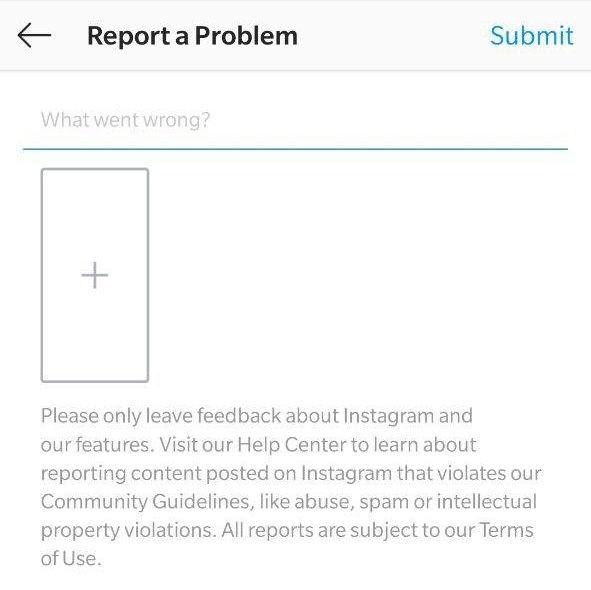
\includegraphics[width=\linewidth]{img/instagram-feedback/instagram-feedback.jpg}
	\caption{Formular aus der Instagram \cite{Instagram} Android App}
	\label{fig:instagram-feedback-example}
\end{wrapfigure}

%Aufgrund dieser Bedingungen werden bei Webprojekten Probleme im Feld erwartet. Zur Behebung dieser Mängel benötigen die Stakeholder Informationen. Für Nutzer gibt es daher oftmals Formulare um diese Auffälligkeiten zu melden (Beispiel siehe rechts). Die Einbindung solcher Formulare ist zeit- und kostengünstig, kann aber nur erfolgreich sein, wenn die Nutzer verständliches und informatives Feedback geben können und wollen.

Diese Hürden für Stakeholder umfassen folgendes:
\begin{enumerate}
	\item Kontextinformationen sind nicht einsehbar und
	\item Nutzerverhalten ist nicht bekannt.
\end{enumerate}

Problemberichte sind eine gängige Wahl, um den Stakeholdern eine  Verständnishilfe zu bieten (vgl. ~\autoref{fig:instagram-feedback-example}). Bettenburg \etal \cite{WhatMakesAGoodBugReport} fanden jedoch bei Problemberichten eine Diskrepanz, zwischen dem was die Stakeholder als hilfreich empfanden und dem was Nutzer ihnen als Bericht lieferten.

Dies lässt folgern, dass die Informationserhebung nicht allein von den Nutzern aus geschehen sollte. Es ist ein übergreifendes Konzept anzustreben, welches die Informationslücke ausgleicht und eine Nachvollziehbarkeit für die Stakeholder ermöglicht.

%\begin{itemize}
%	\item 	Was soll mit der Arbeit erreicht werden? Welche Ziele werden angestrebt?
%			Möglichst kurz und präzise geplante Ergebnisse umreißen. Daran werden
%			Ihre Resultate am Ende gemessen!
%\end{itemize}
\section{Zielsetzung}

\nomenclature[Fachbegriff]{SPA}{Single Page Application}
\nomenclature[Fachbegriff]{DSGVO}{Datenschutz Grundverordnung}

Ziel dieser Arbeit ist es, eine Möglichkeit zu schaffen, dass die Stakeholder die Interaktionen eines Nutzers und das Verhalten einer Webapplikation nachvollziehen können. Dieses Ziel wird unter dem Begriff ``Nachvollziehbarkeit`` zusammengefasst.

Folgende Fragen sollen im Zuge der Ausarbeitung beantwortet werden:

% Feedback von Stephan: Gefällt mir in der neuen Fassung gut. Ggf. kannst du zu 1 noch 2-3 Unterpunkte hinzufügen worauf du genauer eingehen willst -> z.B. Fehler, "Nutzerverhalten" (wie navigiert der User durch die Anwendung), ...

\begin{enumerate}
	\item Was bedeutet Nachvollziehbarkeit?
	\item Warum ist Nachvollziehbarkeit wichtig?
	\item Wie kann eine gute Nachvollziehbarkeit erreicht werden?
	\begin{enumerate}
		\item Was wird hierzu benötigt?
		\item Wie kann Nutzerverhalten nachvollzogen werden?
		\item Wie können Fehler nachgestellt werden?
	\end{enumerate}
	\item Wie ist eine Webapplikation zu erweitern um dies zu erreichen? \\ (Hierbei sollen Projekte von Open Knowledge untersucht werden.)
	\begin{enumerate}
		\item Was für Technologien helfen hierbei?
		\item Was sind die Auswirkungen für den Nutzer?
		\begin{enumerate}
			\item Wird die Leistung der Webapplikation beeinträchtigt?
			\item Wie wird mit seinen Daten umgegangen (Stichwort DSGVO)?
		\end{enumerate}
	\end{enumerate}
\end{enumerate}


\subsection{Abgrenzung}

% Feedback von Christian: ja finde ich auch gut. Ich war zwischendurch am überlegen, in welchem Rahmen man das betrachten kann, da Datenschutz und Datensicherheit ja ein großes Thema ist. Also, ob man da nicht ggf. eine Abgrenzung machen sollte.

Bei der Betrachtung von Webapplikationen, sollen nur jene betrachtet werden, die dynamisch mit JavaScript erzeugt werden - auch Single-Page-Applications (SPAs) genannt.

Bei der Implementierung soll ein Proof-of-Concept (PoC) bzw. eine Demonstration der vorgestellten Methoden und Konzepte erstellt werden. Eine allgemeingültige Lösung übersteigt den Rahmen der Bachelorarbeit und ist nicht anzustreben.

\nomenclature[Fachbegriff]{PoC}{Proof-of-Concept}

Im Zuge der Implementierung der Erweiterung, soll beleuchtet werden, welche Daten erhoben werden und wie mit diesen umgegangen wird. Eine Analyse der Datenverarbeitung in Hinblick auf vollste Konformität mit der DSGVO wird jedoch nicht Bestandteil sein.

\pagebreak

%\begin{itemize}
%	\item 	Wie wird vorgegangen, um das Ziel zu erreichen?
%	\item 	Warum ist die Arbeit so gegliedert, wie sie gegliedert ist?
%	\item 	Welche Aspekte werden nicht behandelt und warum?
%\end{itemize}
\section{Vorgehensweise}

Es ist dem Leser zu vermitteln, was die theoretischen Grundlagen sind und wie die der Nachvollziehbarkeit definiert wird. Es gilt zu erörtern, warum die Nachvollziehbarkeit erstrebenswert ist und wie sehr sie bereits Beachtung findet.

Durch das gewonnene Verständnis über die Ausgangssituation, sind nun Methoden aufzuzeigen, welche eine Nachvollziehbarkeit unterstützen. Methoden wie Fehlerberichte, Logging, Metriken, Monitoring, Tracing und ggf. andere sind zu betrachten.

Auf Basis des detaillierten Verständnisses der Problemstellung und der Methoden wird nun die Erstellung eines Proof-of-Concepts (PoC) Fokus sein. Das PoC erfolgt auf Basis bestehender Webapplikation der Open Knowledge GmbH. Sie soll als Ziel haben, die Nachvollziehbarkeit zu erhöhen.

Zum Abschluss ist ein Fazit zu erstellen. Darin enthalten ist eine kritische Eigenreflexion sowie ein Ausblick, welcher beschreibt, wie das Themengebiet und die erstellte Software voranschreiten könnten.

% Anfangs soll identifiziert werden, was alles für einen Nutzer ein Problem darstellen kann. Es muss sich bei den Problemen nicht nur um Laufzeitfehler o.Ä. handeln, sondern Logikfehler oder auch Verständnisprobleme führen zu einer Einschränkung der Nutzbarkeit. Hier soll eine Analyse aus der Literatur und ggf. einer Umfrage erstellt werden, um daraufhin grobe Problembilder zu klassifizieren.

% Danach soll erörtert werden, welche Ursachen es für häufige Problemszenarien gibt. Darauf aufbauend könnten Aussagen getroffen werden, wie diese Szenarien bereits vorher vermeidet werden können oder die Häufigkeit reduziert werden kann.

%Durch das gewonnene Verständnis über diese Probleme, soll nun ein Konzept erarbeitet werden. Dieses Konzept soll darauf abzielen zu den einzelnen Problembildern jeweils einen Ansatz zu finden, diese aufzuzeigen und den Stakeholdern Informationen zu liefern, die bei der Behebung notwendig sind (bspw. Geräteinformationen, Sitzungsinformationen, Logs, etc.).

% Zunächst soll ein Konzept erstellt werden, welches die Komponenten definiert und beschreibt und die Interaktion zwischen den Komponenten umfasst. Auf Basis der Konzeptes soll nun die Implementierung der Erweiterung erfolgen.

% Da nun ein Basisverständnis gewonnen wurde, sollen etablierte Technologien wie Google Cloud \cite{GoogleCloudErrorReporting}, Dynatrace \cite{DynatraceDigitalExperienceMonitoring}, Sentry \cite{SentryForJavaScript} und LogRocket \cite{LogRocket} näher betrachtet werden. Durch die Erörterung des Stands der Technik sollen folgend Empfehlungen ausgesprochen werden, für welche Projekte welche Technologie oder Kombination von Technologien sinnvoll ist. Sollte keine Technologie als angemessen betrachtet werden, so soll basierend auf den Anforderungen ein Vorschlag gemacht werden, wie so eine Technologie aussehen könnte.

%\newpage

\section{Open Knowledge GmbH}

%{\color{red}TODO: Dieser Abschnitt muss noch überarbeitet werden}

Die Bachelorarbeit wird unter anderem im Rahmen einer Werkstudententätigkeit innerhalb der Open Knowledge GmbH erstellt. Der Standortleiter des Standortes Essen, Dipl. Inf. Stephan Müller, übernimmt die Zweitbetreuung.

Die Open Knowledge GmbH ist ein brancheneutrales mittelständisches Dienstleistungsunternehmen mit dem Ziel bei der Analyse, Planung und Durchführung von Softwareprojekten zu unterstützen. Das Unternehmen wurde im Jahr 2000 in Oldenburg, dem Hauptsitz des Unternehmens, gegründet und beschäftigt heute 74 Mitarbeiter. Mitte 2017 wurde der zweite Standort in Essen eröffnet an dem aktuell 13 Mitarbeiter angestellt sind.

Die Mitarbeiter von Open Knowledge übernehmen in Kundenprojekten Aufgaben bei der Analyse über die Projektziele und der aktuellen Ausgangssituationen, der Konzeption der geplanten Software, sowie der anschließenden Implementierung. Die erstellten Softwarelösungen stellen Individuallösungen dar und werden den Bedürfnissen der einzelnen Kunden entsprechend konzipiert und implementiert. Technisch liegt die Spezialisierung bei der Mobile- und bei der Java Enterprise Entwicklung, bei der stets moderne Technologien und Konzepte verwendet werden. Aufgrund der großen Expertise in den Bereichen Technologien und Konzepte sind sowohl die Geschäftsführer als auch diverse Mitarbeiter der Open Knowledge GmbH als Redner auf Fachmessen wie der Javaland oder Autoren in Fachzeitschriften wie dem Java Magazin vertreten.% \cite{VincentOpenKnowledge} % Auch aufgrund der medialen Präsenz konnte die Open Knowledge GmbH in den letzten Jahre zahlreiche Projekte für namhafte Kunden, wie z.B. Vodafone, die HUK-Coburg, die Daimler AG und die DB Schenker AG übernehmen. \cite{VincentOpenKnowledge}

%Durch das breite Dienstleistungsangebot und die Branchenneutralität übernimmt die Open Knowledge GmbH Projekte aus der Automobilindustrie, der Luft- und Raumfahrt, dem Bankwesen und dem Versicherungswesen innerhalb des nationalen und europäischen Raums.
%
%Entsprechend der Philosophie ``Offenkundig Gut`` und dem Namen des Unternehmens wird stets versucht das benötigte Wissen zur Erstellung und Wartung der Software mit dem Kunden zu teilen, sodass die Kunden nach Abschluss der Projekte in der Lage sind, die Software selbstständig zu Pflegen und die Projektarbeit von OK damit abgeschlossen ist \cite{OpenKnowledgePhilosophie}.

\pagebreak
